 \section{Description and Analysis of the Domain}

Nowadays, we are living in the era of technological progress, where machines get to do the most part of the jobs people once used to do entirely. It is vital to understand and sustain the every day life improvements human kind gets while creating software, instead of using the ancient approach of doing everything individually. Sooner people get that, faster they reach the point when machines are included into the daily routine to complete the tasks that, for a person, would take much more resources. It is the most efficient way for people to save time and money while introducing software for optimization purpose. This means that there is an worldwide tendency for developing smart systems which would eventually replace the unnecessary extra effort made by one or more people involved in a certain process by swapping it with functional products. Here we reach the moment where an informational system becomes more suitable for small, repetitive jobs, in order to ensure some more free hands to take care of complex tasks. 

As mentioned above, passing from traditional methods of building environmental infrastructures to the computerized ones it is not an easy task and the approach has to be a well-defined from the start. Big changes don't always fit perfectly, bringing with them a lot of problems to deal with. That's why, it is important to determine from the beginning the correct manner for defining new standards. Locally speaking, it has been seized a continuously growing interest in determining people to work with software, which is encouraging the technological progress to spread evenly among all the population. The young generation deals better with this phenomenon, while a real challenge is faced to middle age generation. Still, this temporary phase shouldn't be treated as a problem, but as a matter of accommodation.

Diving deeper into the subject, the local educational system gets involved in the discussion. As a matter of fact, the academic structures should be the first ones involved in the transition from standard methodologies to the progressive ones. It is already observed a constant aspiration and sympathy for new technologies which implies the reorganization of the academic structures. This means that people already reached the moment when are ready to bring software products in universities in order to optimize the routine processes which they are responsible for accomplishing.  This is a big step that has to be adjusted properly to the university's needs. 

inClass is the software product that comes with a project in development and a prototype to fix an existing problem in universities. At the same time, it represents a small change for the academic infrastructure, given the fact that is easy to implement, use and maintain, while the results are consistently improved. So, such a product brings with it a lot of benefits for its users:
\begin{itemize}
\item Helps in improving user's time management;
\item Brings additional flexibility by saving user's time during breaks;
\item It is practical in use and easy to handle;
\item Can be easily accessed only by having a smartphone and internet connection.
\end{itemize}

\subsection{The workflow of the system}
In order to be able to access the inClass application, a user should create an account first. Given the fact that there are two types of user, the registration modality differs for each of them. The registration for students is a traditional one, by reaching the domain of the application and request a new account. At the registration stage, the student will be asked to identify himself/herself by specifying their study group. The student will be able to select its own group, ensuring this way a proper generation of his/her schedule. After log in, the student will be able to visualize his/her current timetable, depending on the current day. The application compares the general current day from the set up date and matches it with the label "Day", that every course has specified at creation. As mentioned above, there is a third-party user, the administrator, whose task is to populate the database with records, which are the courses, in our case and take care of the maintenance of the database during the current semester. If any changes appear in the general timetable, the administrator is able to introduce all the changes by editing the courses in cause. 

Speaking about the other type of user, the teacher, there is a different procedure defined for him/her in order to get an account. For security reasons, the accounts for teachers are created by the admin. He is the one that directly generates the teacher's accounts and is also responsible for the secure credentials sharing with the teachers in discussion. The decision of admin taking care of teacher's accounts was made assuming that the courses are linked with the teacher. Because of that, the courses' moment of creation is dependent on the teacher's moment of account creation. So, for avoiding other conflicts, the system was developed based on the assumption that the teachers already exist in the database when the courses are created. 

Another moment that gives additional credit to the discussed product is the fact that inClass is a flexible application, developed for a general purpose. Meaning that, even if it was first designed to forehead a specific problem appeared at a specific university, it's still independent from usability point of view. So, if any other university is desiring to implement in their administrative infrastructure this product, there are no problems with that, because the application permits multiple records of different universities. The only moment that should be taken in consideration is the database capacity, that should have proper dimensions for data insertions. At this point, the database population is handled by systematic updates, which assume that at every semester end, all the records from the database are destroyed (because the timetables also change) and new records are created when a new semester begins. Assuming that the project is in its early development stage, there are no archives of old data in the system. so, once a course is not valid anymore, it is simply erased. Still, this can not be considered as a flaw of the system, since once passed a semester, the old record are of no actual use.

\subsection{Similar products on the market}
The idea of creating the discussed application came from the possibility of using and testing another existing product on the market during some time. Assuming that, in order to create a good software, it is necessary to make a market research and find similar solutions to the problems that are being solved by that software, making a connection between the original system and the missing one from the local academic infrastructure was quite obvious. The initial product, which served as inspiration, was implemented as a general platform for one of the foreign faculties in Europe. inClass can be considered as a child of the original application because it covers only a part of its initial functionality. If to discuss the original platform, it covered almost completely the academic infrastructure of the mentioned faculty. Also, another thing that should be taken in consideration is the fact that the foreign faculty had different rules for timetable creation, implying student's decision of the courses to be attended. All the courses and their description was available on the platform and contained details about those courses like subjects to be discussed, practical assignments, all kinds of feedback, like received marks during the semester. So, once a student was decided about the courses to attend, the system generated his/her individual timetable, according to the subscriptions the student made. 

Making a parallel to the local universities, students don't get the chance to choose what the want to learn from a proposed list of subject because the curriculum is already established by the Ministry of Education. That's why, transposing the original platform for the local needs, the task gets easier with the fixed curriculum. Yet, the rest of the application can be considered a prototype of the original system.

Another local example, that was already implemented in the academic structures is the Moodle learning platform. Since the beginning, Moodle was designed to provide educators, administrators and learners with a single robust, secure and integrated system to create personalized learning environments.Moodle is also web-based and so can be accessed from anywhere in the world. With a default mobile-compatible interface, the content on the Moodle platform is easily accessible and consistent across different web browsers and devices.It has a simple interface, drag-and-drop features and well-documented resources along with ongoing usability improvements. It is a good solution for course content integration, but not for dealing with course management. Still, the project has an open-source approach, meaning that it is continually being reviewed and improved on to suit the current and evolving needs of its users, \cite{Moodle}. 

For future implementation, using Moodle's API for integration with the currently discussed product would constitute an even more powerful tool for academic activities. It would cover all the basic functionality needed to overpass the obsolete current methodology for teaching and learning purposes. 

\subsection{The development environment}
A framework is a program, set of programs and code library that writes most of the application for the developer. While using a framework, the main job is to write the parts of the application that make it do the specific things the developer wants. When writing a Rails application, leaving aside the configuration and other housekeeping chores,there are 3 primary tasks to perform:
\begin{itemize}
\item Describe and model the application's domain - The domain is the universe of the application. In this case, the domain represents an application that would allow the monitoring of personal study timetable. So here has to be established what's in it, what entities exist in this universe and how the items in it relate to each other. This is equivalent to modeling a database structure to keep the entities and their relationship.
\item Specify what can happen in this domain - The domain model is static; it has to become dynamic. Students  and teachers can register fin order to view their timetables. So, it is necessary to identify all the possible scenarios or actions that the elements of the domain can participate in.

\item Choose and design the publicly available views of the domain − At this point, thinking in Web-browser terms can start. Once it's decided that the domain has students and teachers, and that they can register for viewing timetables, some components like a home page, a registration page, and a log in page can be envisioned. Each of these pages, or views, shows the user how things stand at a certain point.
\end{itemize}

Based on the above three tasks to be accomplished, Ruby on Rails framework was chosen for the development of the discussed  application, assuming that it suites the best from implementation point of view. 

\subsubsection{Back-end implementation: Ruby on Rails}
For implementing the idea of the inClass project, Ruby language was chosen, Ruby being a general-purpose programming language, best known for its use in web programming. It is known among programmers for a brief, uncluttered syntax that doesn't require a lot of extra punctuation. Compared to Java, Ruby is streamlined, with less code required to create basic structures such as data fields. Ruby's key advantage is RubyGems, the package manager that makes it easy to create software libraries (gems) that extend Ruby. RubyGems provides a simple system to install gems. Anyone can upload a gem to the central RubyGems website, making the gem immediately available for installation and building complex websites by anyone, \cite{RoR}.

The application was built on Rails framework,which is also written in Ruby and is a web application framework. Rails is a MVC framework, providing default structures for a database, a web service, and web pages. It encourages and facilitates the use of HTML, CSS and JavaScript for display and user interfacing. In a default configuration, a model in the Ruby on Rails framework maps to a table in a database and to a Ruby file. For example, the model class Student is defined in the file 'student.rb' in the app/models directory, and linked to the table 'students' in the database. 

A controller is a server-side component of Rails that responds to external requests from the web server to the application, by determining which view file to render. The controller may also have to query one or more models directly for information and pass these on to the view. A controller may provide one or more actions. In Ruby on Rails, an action is typically a basic unit that describes how to respond to a specific external web-browser request. Also for the controller/action to be accessible for external web requests, it is necessary a corresponding route to be mapped to it. A view in the default configuration of Rails is an .erb file, evaluated and converted to HTML at run-time, \cite{RoR2}.

inClass application was built on Ruby on Rails because this environments offers all the suitable components and tools for achieving an optimal result in a minimal period of time. Several RubyGems were used in order to reach additional functionality of the final product. One of the main RubyGems used in the project was Devise, which is a flexible authentication component for Rails, bringing a complete MVC solution based on Rails engine, allowing to have multiple models signed in at the same time. Having the possibility to use the RubyGems made possible the inclusion of Hierapolis theme as front-end on the administration side of the application. 

\subsubsection{Model-View-Controller architecture inside Rails}
The MVC principle divides the work of an application into three separate, but closely cooperating subsystems. In \autoref{fig:MVC-Rails} is represented the schematic diagram of Rails components interacting according to the MVC pattern:

\begin{figure}[H]
\centering
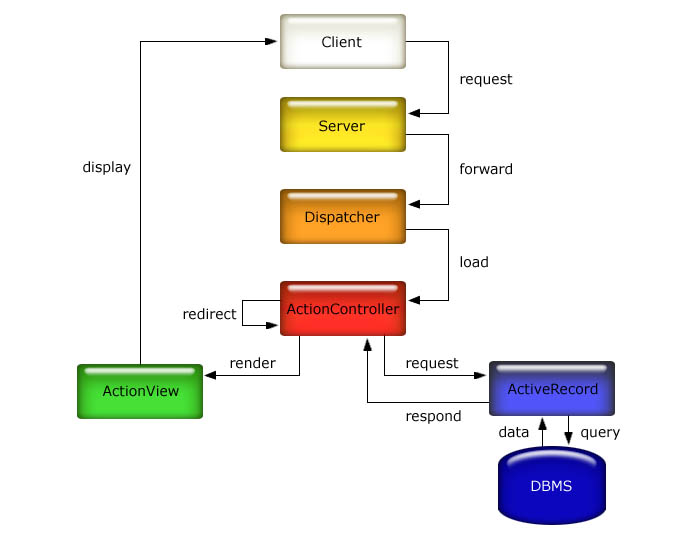
\includegraphics[width=12cm]{Chapter1/mvc-rails.jpg}
\caption{MVC pattern integration with Rails, \cite{mvc}}
\label{fig:MVC-Rails}
\end{figure}

The Model maintains the relationship between the objects and the database, while handling validation, association, transactions, and more. This subsystem is implemented in Active Record library, which provides an interface and binding between the tables in a relational database and the Ruby program code that manipulates database records. Ruby method names are automatically generated from the field names of database tables.

The View is a presentation of data in a particular format, triggered by a controller's decision to present the data. They are script-based template systems, which are easy to integrate with JavaScript technology. This subsystem is implemented in Action View library, which is an Embedded Ruby (ERb) based system for defining presentation templates for data presentation. Every web connection to a Rails application results in the displaying of a view.

The Controller is the facility within the application that directs traffic, on the one hand, querying the models for specific data and on the other hand, organizing that data (searching, sorting, messaging it) into a form that fits the needs of a given view. This subsystem is implemented in Action Controller, which is a data broker sitting between Active Record (the database interface) and Action View (the presentation engine), \cite{mvc2}.

\subsubsection{Handling Models with Active Record}
Active Record is the \textbf{M} in MVC - the model - which is the layer of the system responsible for representing business data and logic. Active Record facilitates the creation and use of business objects whose data requires persistent storage to a database. It is an implementation of the Active Record pattern which itself is a description of an Object Relational Mapping system, \cite{activeRecord}. 

Object-Relational Mapping, commonly referred to as its abbreviation ORM, is a technique that connects the rich objects of an application to tables in a relational database management system. Using ORM, the properties and relationships of the objects in an application can be easily stored and retrieved from a database without writing SQL statements directly and with less overall database access code\cite{orm}.

Active Record gives several mechanisms, the most important being the ability to:
\begin{itemize}
\item Represent models and their data;
\item Represent associations between these models;
\item Represent inheritance hierarchies through related models;
\item Validate models before they get persisted to the database;
\item Perform database operations in an object-oriented fashion, \cite{activeRecord-orm}.
\end{itemize}

When writing applications using other programming languages or frameworks, it may be necessary to write a lot of configuration code. This is particularly true for ORM frameworks in general. However, if the conventions adopted by Rails are followed, there is no need to write configuration when creating Active Record models. The idea is that if the application is configured in the very same way most of the time, then this should be the default way. Thus, explicit configuration would be needed only in those cases where a developer can't follow the standard convention, \cite{conventions}.

\subsubsection{Front-end implementation: Bootstrap, CSS and JavaScript }
For the front-end development of the application, Bootstrap was the main tool to be used. Bootstrap is a free and open-source front-end web framework for designing websites and web applications. It contains HTML and CSS based design templates for typography, forms, buttons, navigation and other interface components, as well as JavaScript extensions. Bootstrap includes a responsive, mobile first fluid grid system that appropriately scales up to 12 columns as the device or viewport size increases. It includes predefined classes for easy layout options, as well as powerful mixins for generating more semantic layouts. In addition to the regular HTML elements, Bootstrap contains other commonly used interface elements. These include buttons with advanced features (grouping of buttons or buttons with drop-down option, horizontal and vertical tabs, navigation, pagination, etc.), labels, advanced typographic capabilities, thumbnails, warning messages and a progress bar. The components are implemented as CSS classes, which must be applied to certain HTML elements in a page, \cite{bootstrap}.

Cascading Style Sheets (CSS) is a style sheet language used for describing the presentation of a document written in a markup language. Although, most often, it is used to set the visual style of web pages  written in HTML, for the inClass project, the CSS files were related to files written in HAML (a revised version of HTML). CSS is designed primarily to enable the separation of document content from document presentation, including aspects such as the layout, colors, and fonts. This separation can improve content accessibility, provide more flexibility and control in the specification of presentation characteristics and reduce complexity and repetition in the structural content, \cite{css}.

Using sprinkles of JavaScript throughout a Rails application is almost inevitable if it is necessary to isolate code to only run specified pages. JavaScript can also make requests to the server, and parse the response. It also has the ability to update information on the page. Combining these two powers, a JavaScript writer can make a web page that can update just parts of itself, without needing to get the full page data from the server, \cite{js}. This is exactly the case where JavaScript code was used in the currently discussed application. 